% ============================================================================
% §2.3 Kết quả — 5 bảng + 2 figure key, ~1.8 trang
% ============================================================================

\subsection{Kết quả}
\label{sec:results}

\subsubsection{Kiểm định đơn chiều, độ tin cậy và độ phù hợp các mô hình LSEM}

\textit{Tính đơn chiều} của ngân hàng câu hỏi được đánh giá bằng phân tích nhân tố khám phá (EFA) + biểu đồ giá trị riêng (Hình~\ref{fig:scree}), tương tự bước kiểm tra giả định đơn chiều trước khi chọn mô hình IRT cho đề kiểm tra Toán THPT trong \cite{buhay2026shstat}. Mặc dù tỷ trọng phương sai chung (ECV) chỉ đạt 0{,}56--0{,}68 (chưa đạt ngưỡng nghiêm ngặt 0{,}80 của đơn chiều thuần tuý), tỷ số giá trị riêng \(\lambda_1/\lambda_2 = 2{,}8\)--6{,}0 cho thấy \emph{nhân tố thứ nhất chiếm ưu thế rõ rệt}; điều này biện minh cho việc sử dụng 1PL --- vốn được biết là robust với sai lệch nhẹ khỏi đơn chiều thuần tuý. Khối~12 có ưu thế đơn chiều mạnh nhất (\(\lambda_1/\lambda_2 = 6{,}0\)), phù hợp với việc khối 12 cũng cho ước lượng \(\hat\theta\) tin cậy nhất ở các phân tích phía sau.

\textit{Độ tin cậy} của \(\hat{\theta}\) được tính theo công thức \(\rho = 1 - \overline{\seit^2}/\widehat{\Var}(\hat\theta)\), đạt 0{,}687 / 0{,}746 / 0{,}814 lần lượt cho ba khối. Khối~10 nằm ngay dưới ngưỡng thông thường (\(\rho \ge 0{,}70\)) --- đây là điểm cần lưu ý khi triển khai các ứng dụng ở cấp cá nhân cho khối này. Tất cả sáu mô hình LSEM (LGCM và LCSM cho ba khối) đều đạt \textit{độ phù hợp} tốt với CFI \(> 0{,}99\), RMSEA \(< 0{,}031\) và SRMR \(< 0{,}017\) (Bảng~\ref{tab:rho_fit}).

\begin{figure}[H]
\centering
% --- Bảng 2 (gộp cùng Hình 3 — cùng nói về chất lượng đo lường) ---
\captionof{table}{Độ tin cậy $\rho$ của $\hat\theta$ và chỉ số độ phù hợp của LGCM/LCSM, theo khối.}
\label{tab:rho_fit}
\footnotesize
\begin{tabular}{l rr  rrrrr  rrrrr}
\toprule
 & \multicolumn{2}{c}{\textbf{Đo lường}} & \multicolumn{5}{c}{\textbf{LGCM}} & \multicolumn{5}{c}{\textbf{LCSM}} \\
\cmidrule(lr){2-3}\cmidrule(lr){4-8}\cmidrule(lr){9-13}
\textbf{Khối} & \textbf{$\overline{\seit^2}$} & \textbf{$\rho$} & \textbf{$\chi^2$} & \textbf{df} & \textbf{CFI} & \textbf{RMSEA} & \textbf{SRMR} & \textbf{$\chi^2$} & \textbf{df} & \textbf{CFI} & \textbf{RMSEA} & \textbf{SRMR} \\
\midrule
10 & 0{,}261 & 0{,}687 & 17{,}08 & 5 & 0{,}996 & 0{,}019 & 0{,}011 &  7{,}11 & 2 & 0{,}998 & 0{,}020 & 0{,}008 \\
11 & 0{,}295 & 0{,}746 & 38{,}45 & 5 & 0{,}991 & 0{,}031 & 0{,}017 &  6{,}81 & 2 & 0{,}999 & 0{,}019 & 0{,}007 \\
12 & 0{,}206 & 0{,}814 & 32{,}50 & 5 & 0{,}997 & 0{,}023 & 0{,}011 & 15{,}20 & 2 & 0{,}998 & 0{,}025 & 0{,}010 \\
\bottomrule
\end{tabular}
\par\vspace{4pt}
% --- Hình 3 (Scree) ---
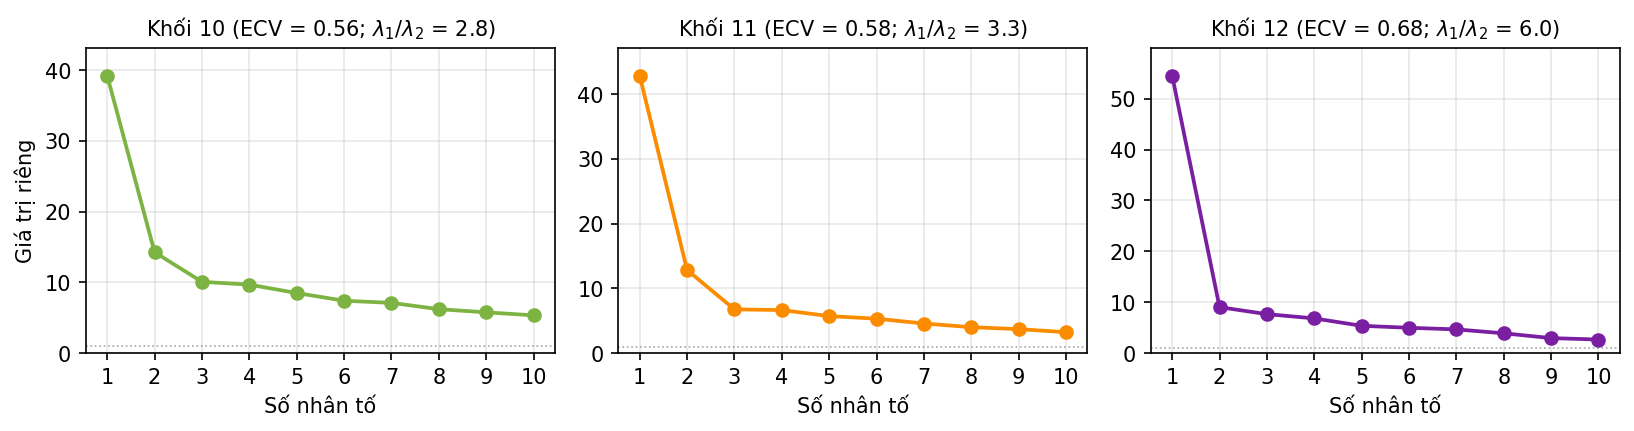
\includegraphics[width=\linewidth]{scree_plots.png}
\captionof{figure}{Biểu đồ giá trị riêng (\emph{scree plot}) theo khối. ECV: tỷ trọng phương sai chung; $\lambda_1/\lambda_2$: tỷ số nhân tố 1 trên nhân tố 2 (càng lớn càng đơn chiều).}
\label{fig:scree}
\end{figure}

\subsubsection{Quỹ đạo tăng trưởng theo khối: từ đuổi kịp đến ổn định}

Hệ số tăng trưởng LGCM dương ở cả ba khối, song độ lớn khác nhau rõ rệt: khối~11 tăng nhanh nhất (\(s = 0{,}028\) logit mỗi đợt, khoảng tin cậy không chứa 0), khối~10 ở mức trung bình (\(s = 0{,}015\)), khối~12 gần như đi ngang (\(s = 0{,}006\)). Hệ số ghép cặp \(\beta\) của LCSM (Hình~\ref{fig:lgcmlcsm}, ô phía trên bên phải) cho thấy một khuôn mẫu thay đổi rất rõ rệt theo khối lớp:
\begin{itemize}
  \item Khối~10: \(\beta = -0{,}069\); khoảng tin cậy 95\% \([-0{,}119,\ -0{,}022]\) \textbf{không chứa 0} --- cơ chế đuổi kịp có ý nghĩa thống kê.
  \item Khối~11: \(\beta = -0{,}043\); khoảng tin cậy 95\% chứa 0 --- xu hướng đuổi kịp đã suy yếu, không còn ý nghĩa thống kê.
  \item Khối~12: \(\beta = +0{,}002\); khoảng tin cậy 95\% chứa 0 và đối xứng quanh 0 --- trạng thái ổn định, không còn ghép cặp.
\end{itemize}

Diễn giải thực tiễn: ở khối~10, một học sinh có \(\theta_{t-1} = -1\) logit (yếu hơn trung bình khối khoảng một độ lệch chuẩn) được kỳ vọng tăng thêm \(|\beta| \cdot 1 \approx 0{,}07\) logit so với học sinh ở mức trung bình ở đợt tiếp theo --- tương đương khoảng 1{,}7\% xác suất trả lời đúng một câu có độ khó trung bình. Hiệu ứng này cộng dồn qua nhiều đợt: sau 5 đợt đánh giá, học sinh yếu được dự đoán đuổi kịp xấp xỉ 0{,}3 logit, tức khoảng 7\% xác suất đúng một câu trung bình so với học sinh khá cùng khối.

\begin{figure}[H]
\centering
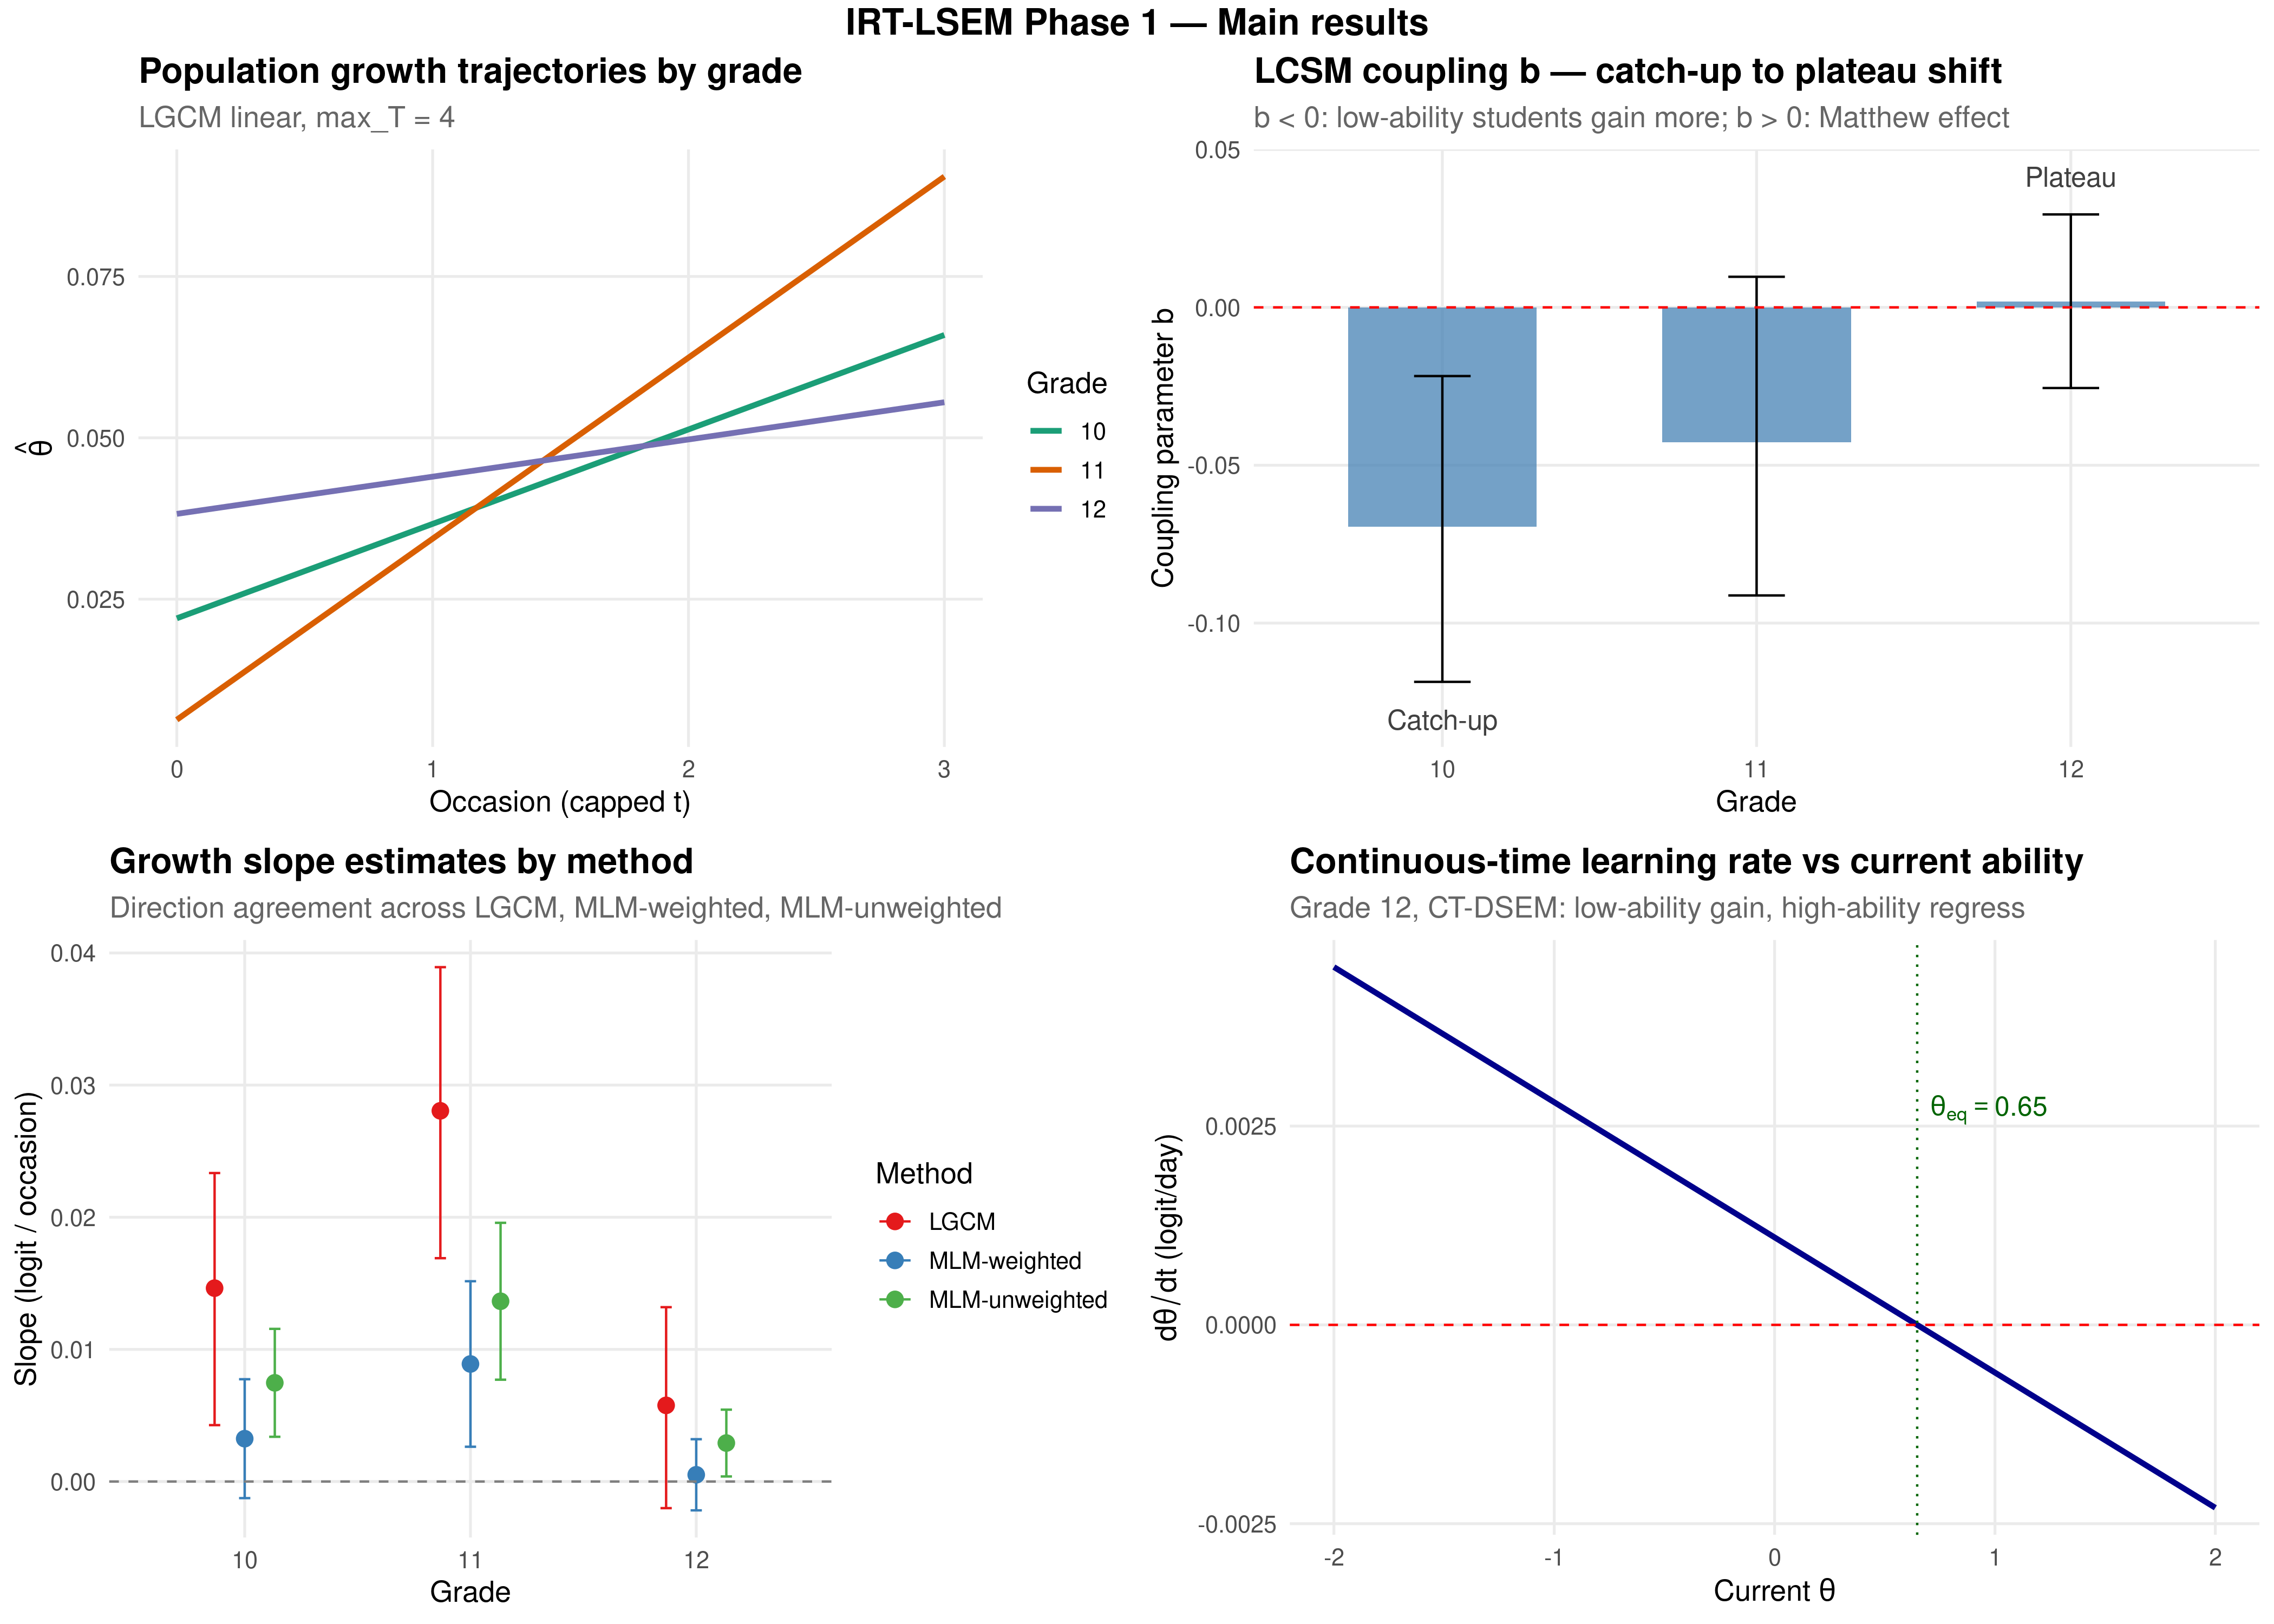
\includegraphics[width=0.95\linewidth]{main_results.png}
\caption{Bốn kết quả chính: quỹ đạo LGCM, hệ số ghép cặp \(\beta\) LCSM, độ dốc đồng dấu từ ba phương pháp, và tốc độ học CT-DSEM ở khối 12 (khối 10/11/12 = xanh lá / cam / tím).}
\label{fig:lgcmlcsm}
\end{figure}

\subsubsection{So sánh thống kê giữa mô hình động và mô hình tĩnh cơ sở}

So sánh AIC/BIC và Kiểm định Tỷ số Hợp lý (Likelihood Ratio Test, LRT) giữa mô hình tĩnh (chỉ có hệ số chặn) và mô hình động (hệ số chặn cộng độ dốc) khẳng định ưu thế áp đảo của mô hình động (Bảng~\ref{tab:lrt}). \(\Delta\)AIC ở mức 82--167 vượt xa ngưỡng thông thường 10 (mức bằng chứng mạnh); giá trị \(p\) của LRT nhỏ hơn \(10^{-19}\) ở cả ba khối và đạt mức \(3 \times 10^{-37}\) ở khối~12.

\begin{table}[H]
\centering\small
\caption{So sánh mô hình tĩnh (chỉ có chặn) với mô hình động (chặn + độ dốc).}
\label{tab:lrt}
\begin{tabular}{lrrrr}
\toprule
\textbf{Khối} & \textbf{$\Delta$AIC} & \textbf{$\Delta$BIC} & \textbf{LRT $\chi^2$ (df=3)} & \textbf{$p$-value} \\
\midrule
10 &  82 &  57 &  87{,}8 & $6{,}5 \times 10^{-19}$ \\
11 &  92 &  67 &  97{,}7 & $4{,}9 \times 10^{-21}$ \\
12 & 167 & 140 & 172{,}9 & $3{,}0 \times 10^{-37}$ \\
\bottomrule
\end{tabular}
\end{table}

\subsubsection{CT-DSEM khối 12: động lực chậm về điểm cân bằng}

Trên tập con khối~12 có \(T_i \ge 15\) (\(N = 460\) học sinh), các tham số của mô hình Ornstein--Uhlenbeck (Bảng~\ref{tab:ctdsem}) cho thấy \(\varphi = -0{,}0017\) (khoảng tin cậy âm, động lực quay về điểm cân bằng), điểm cân bằng dài hạn \(\theta_{\mathrm{eq}} = +0{,}65\) logit (tương ứng \(\approx 66\%\) xác suất trả lời đúng câu trung bình) và bán chu kỳ 408 ngày (vượt một năm học). Tại \(\theta = -1\), tốc độ kỳ vọng đạt \(+0{,}0028\) logit/ngày, tương đương khoảng \(+0{,}25\) logit/học kỳ; tại \(\theta = +1\), tốc độ là \(-0{,}0006\) logit/ngày --- học sinh giỏi có hiện tượng hồi quy về trung bình (\emph{regression to the mean}) nhẹ ngay trong khối~12.

\begin{table}[H]
\centering\small
\caption{Tham số CT-DSEM ở cấp tổng thể (khối 12, $T_i \ge 15$, $N = 460$).}
\label{tab:ctdsem}
\begin{tabular}{lrr}
\toprule
\textbf{Tham số} & \textbf{Ước lượng} & \textbf{CI 95\%} \\
\midrule
$\varphi$ (hệ số trôi)              & $-0{,}0017$ & $[-0{,}0027, -0{,}0010]$ \\
$\mu \varphi$ (hằng số tích phân)   & $+0{,}0011$ & $[+0{,}0006, +0{,}0016]$ \\
$\sigma$ (khuếch tán)               & $0{,}046$   & $[0{,}041, 0{,}053]$ \\
phương sai quan sát $\sigma_\varepsilon^2$ & $0{,}572$ & $[0{,}562, 0{,}582]$ \\
$\theta_{\mathrm{eq}}$              & $+0{,}65$   & --- \\
bán chu kỳ (ngày)                   & 408         & --- \\
\bottomrule
\end{tabular}
\end{table}

\subsubsection{Tác dụng làm trơn của bộ lọc Kalman}

Bộ lọc Kalman cục bộ giúp giảm phương sai sai số đo lường EAP từ 32{,}0\% đến 41{,}2\% mà không cần tăng số câu hỏi khảo sát (Bảng~\ref{tab:ks}, Hình~\ref{fig:kalman}). Phương sai trạng thái ước lượng được \(\hat q_g\) phản ánh biến thiên \emph{thực} của năng lực giữa các đợt đánh giá: khối~11 dao động lớn nhất (\(\sqrt{q} \approx 0{,}86\) logit), gợi ý rằng đây là giai đoạn năng lực biến động mạnh nhất trong ba khối THPT --- nguyên nhân cụ thể (cường độ luyện tập, áp lực thi cử, hay đặc trưng nội dung môn học) cần các nghiên cứu mở rộng để xác định.

\begin{figure}[H]
\centering
\begin{minipage}[c]{0.50\linewidth}
  \centering\footnotesize
  \captionof{table}{Hiệu quả của bộ lọc Kalman: $\overline{\seit}$ giảm và $\hat q_g$ theo khối.}
  \label{tab:ks}
  \resizebox{\linewidth}{!}{%
  \begin{tabular}{lrrrr}
  \toprule
  \textbf{Khối} & \textbf{$\overline{\seit}$ thô} & \textbf{$\overline{\seit}$ làm trơn} & \textbf{Giảm \%} & \textbf{$\hat q_g$} \\
  \midrule
  10 & 0{,}499 & 0{,}387 & 41{,}2 & 0{,}444 \\
  11 & 0{,}527 & 0{,}433 & 34{,}3 & 0{,}734 \\
  12 & 0{,}442 & 0{,}369 & 32{,}0 & 0{,}620 \\
  \bottomrule
  \end{tabular}%
  }
\end{minipage}\hfill
\begin{minipage}[c]{0.48\linewidth}
  \centering
  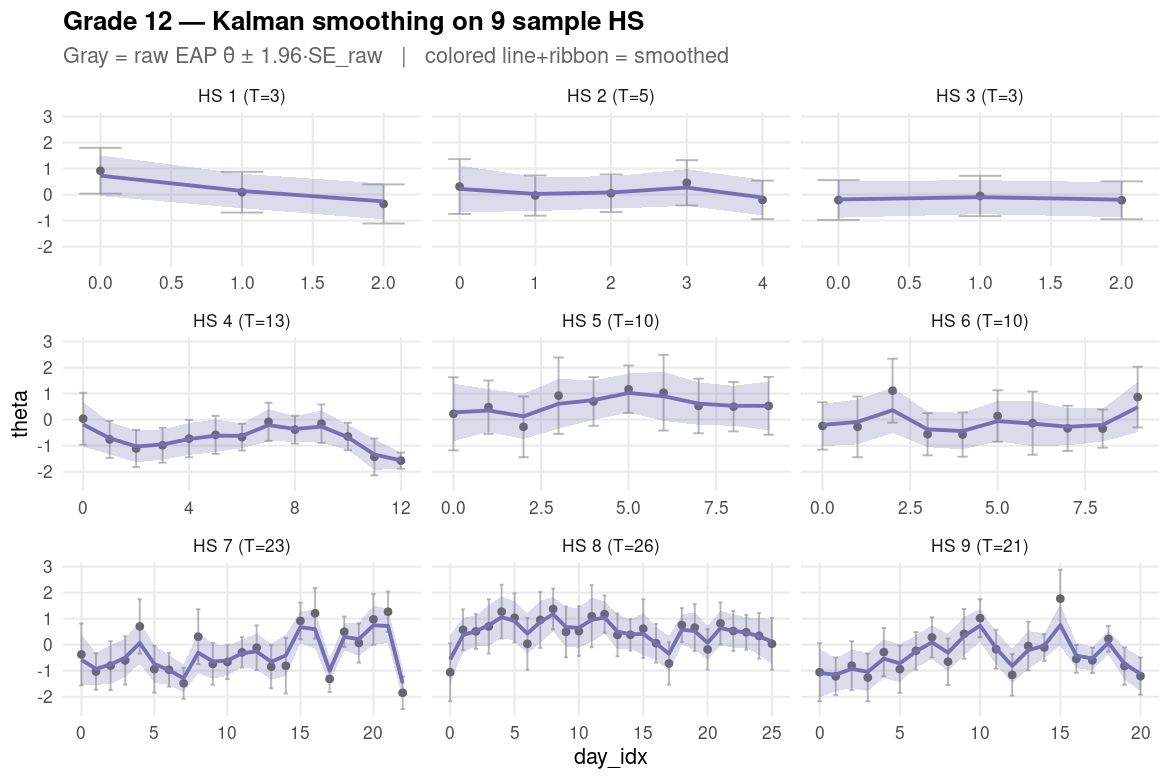
\includegraphics[width=\linewidth]{kalman_overlay_g12.png}
  \captionof{figure}{Chín học sinh khối 12 (ẩn danh): chấm xám = $\hat\theta$ EAP thô, đường liền = quỹ đạo Kalman.}
  \label{fig:kalman}
\end{minipage}
\end{figure}

\subsubsection{Ứng dụng: cảnh báo sớm và gợi ý câu hỏi}

Trên quỹ đạo đã làm trơn, tổng tỷ lệ học sinh bị đánh dấu tăng dần từ khối 10 lên khối 12 (từ 14{,}4\% lên 22{,}3\%; Bảng~\ref{tab:warning}). Nhóm học sinh thoả mãn đồng thời cả hai tiêu chí (tốc độ tăng trưởng thấp và xuất hiện bước giảm đột ngột) duy trì ở mức 3{,}5--5{,}7\% qua ba khối --- đây là tập học sinh cần được giáo viên ưu tiên rà soát thủ công.

Đối với bài toán gợi ý câu hỏi (B7b), 100\% các câu được khuyến nghị có \(|b - \hat\theta_{i,T}| < 0{,}5\) (150 hàng minh hoạ, ứng với 10 học sinh đại diện $\times$ 5 câu $\times$ 3 khối). Tỷ lệ này chủ yếu phản ánh \emph{mật độ cao của ngân hàng câu hỏi} ở vùng độ khó trung bình (Hình~\ref{fig:diff_dist}) chứ không phải đặc thù riêng của thuật toán; đóng góp của bài nằm ở chỗ gợi ý được căn cứ trên quỹ đạo đã làm trơn (phản ánh xu thế gần đây của học sinh) thay vì dựa trên một ước lượng \(\hat\theta\) tĩnh duy nhất.

\begin{figure}[H]
\centering
% --- Bảng 6 ---
\captionof{table}{Số học sinh được cảnh báo sớm theo khối. Cột ``Cả hai'': học sinh thoả mãn đồng thời cả hai tiêu chí (tốc độ tăng trưởng thấp và bước giảm đột ngột).}
\label{tab:warning}
\small
\begin{tabular}{lrrr rrr}
\toprule
\textbf{Khối} & \textbf{$N$ đủ điều kiện} & \textbf{Tổng đánh dấu} & \textbf{\%} & \textbf{Chỉ độ dốc} & \textbf{Chỉ bước giảm} & \textbf{Cả hai} \\
\midrule
10 &  6{.}285 &   905 & 14{,}4 & 411 &   276 & 218 \\
11 &  6{.}740 & 1{.}357 & 20{,}1 & 293 &   683 & 381 \\
12 & 10{.}440 & 2{.}325 & 22{,}3 & 557 & 1{.}281 & 487 \\
\bottomrule
\end{tabular}
\par\vspace{4pt}
% --- Hình 6 (Phân phối độ khó) — dùng layout 3-panel ngang ---
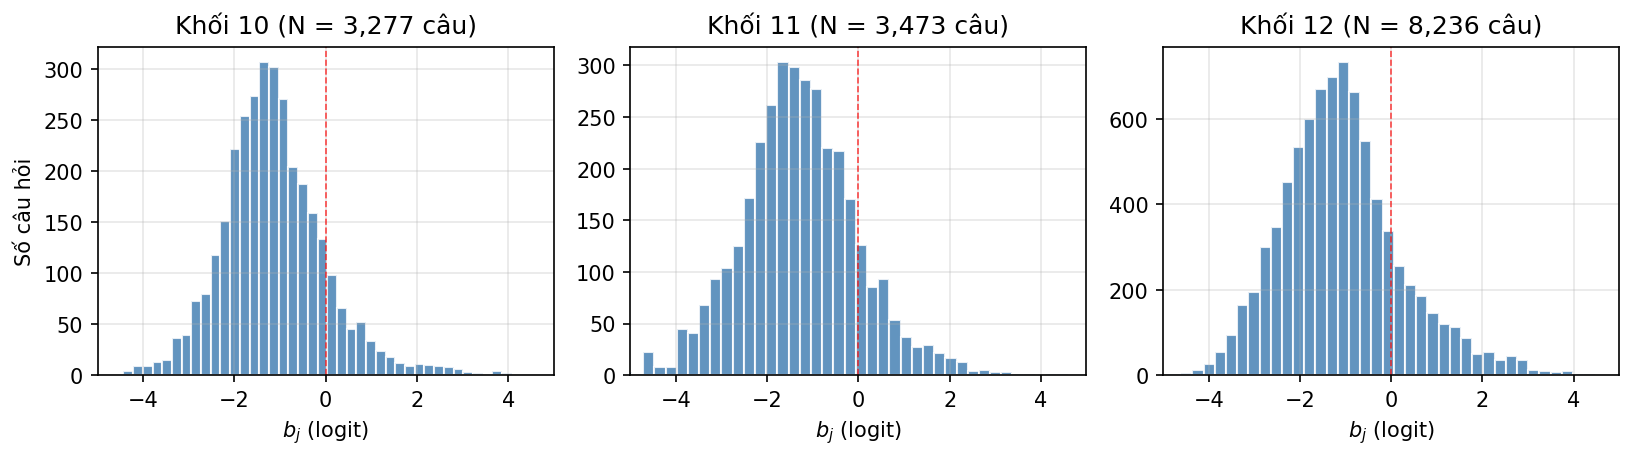
\includegraphics[width=0.95\linewidth]{difficulty_dist_all_grades.png}
\captionof{figure}{Phân phối độ khó $b_j$ theo khối (đường đứt nét đỏ: $b = 0$).}
\label{fig:diff_dist}
\end{figure}
